\begin{figure}
  \centering 
  \begin{subfigure}[b]{0.45\textwidth}
    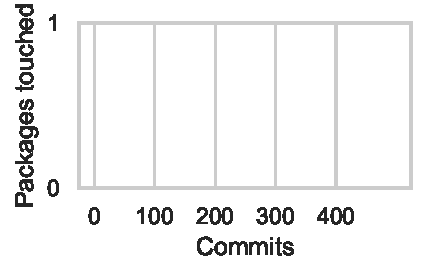
\includegraphics[width=\textwidth]{sections/results/packages/time_series_components_touched.packages.transient.founder.commits_500.pdf}
    \caption{Transient founder (n=206, $\mu$=1.0, median=1.0 \& std=0.0)}
    \label{figure.sections/results/packages/time_series_components_touched.packages.transient.founder.commits_500.pdf}
  \end{subfigure}
  \begin{subfigure}[b]{0.45\textwidth}
    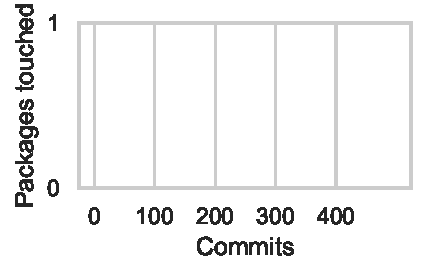
\includegraphics[width=\textwidth]{sections/results/packages/time_series_components_touched.packages.transient.later.joiner.commits_500.pdf}
    \caption{Transient later joiner (n=15304, $\mu$=1.0, median=1.0 \& std=0.0)}
    \label{figure.sections/results/packages/time_series_components_touched.packages.transient.later.joiner.commits_500.pdf}
  \end{subfigure}
\vspace{3mm}
  \begin{subfigure}[b]{0.45\textwidth}
    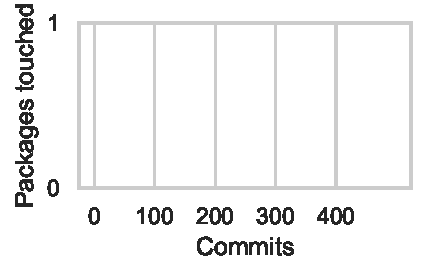
\includegraphics[width=\textwidth]{sections/results/packages/time_series_components_touched.packages.moderate.founder.commits_500.pdf}
    \caption{Moderate founder (n=41, $\mu$=1.0, median=1.0 \& std=0.0)}
    \label{figure.sections/results/packages/time_series_components_touched.packages.moderate.founder.commits_500.pdf}
  \end{subfigure}
  \begin{subfigure}[b]{0.45\textwidth}
    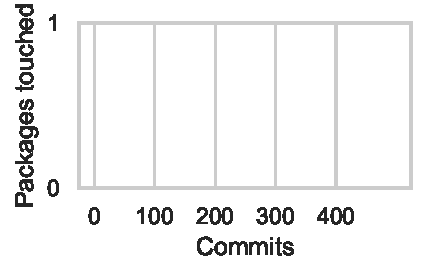
\includegraphics[width=\textwidth]{sections/results/packages/time_series_components_touched.packages.moderate.later.joiner.commits_500.pdf}
    \caption{Moderate later joiner (n=646, $\mu$=1.0, median=1.0 \& std=0.0)}
    \label{figure.sections/results/packages/time_series_components_touched.packages.moderate.later.joiner.commits_500.pdf}
  \end{subfigure}
\vspace{3mm}
  \begin{subfigure}[b]{0.45\textwidth}
    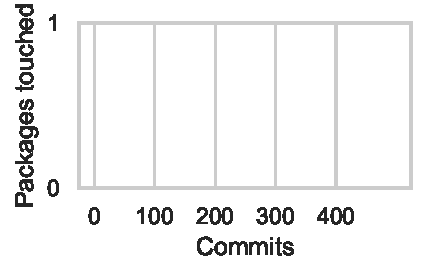
\includegraphics[width=\textwidth]{sections/results/packages/time_series_components_touched.packages.sustained.founder.commits_500.pdf}
    \caption{Sustained founder (n=34, $\mu$=1.0, median=1.0 \& std=0.0)}
    \label{figure.sections/results/packages/time_series_components_touched.packages.sustained.founder.commits_500.pdf}
  \end{subfigure}
  \begin{subfigure}[b]{0.45\textwidth}
    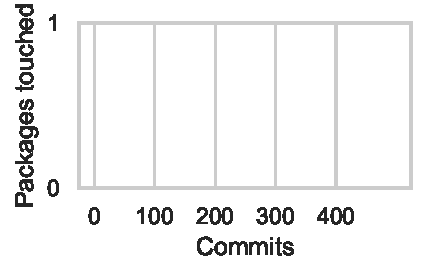
\includegraphics[width=\textwidth]{sections/results/packages/time_series_components_touched.packages.sustained.later.joiner.commits_500.pdf}
    \caption{Sustained later joiner (n=203, $\mu$=1.0, median=1.0 \& std=0.0)}
    \label{figure.sections/results/packages/time_series_components_touched.packages.sustained.later.joiner.commits_500.pdf}
  \end{subfigure}
\caption{A time series for the all commits, excluding transient, with the average mean (blue line), packages touched (y-axis) against the number of commits (x-axis) for six (6) developer categories. Green is the standard deviation above the mean, and pink is the standard deviation below the mean.} 
\end{figure}
\clearpage 
\begin{figure}
  \centering 
  \begin{subfigure}[b]{0.45\textwidth}
    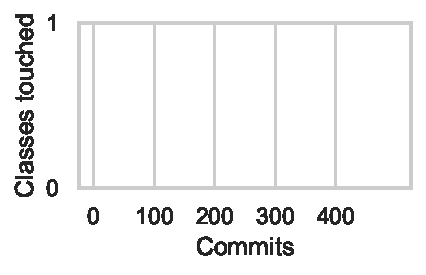
\includegraphics[width=\textwidth]{sections/results/classes/time_series_components_touched.classes.transient.founder.commits_500.pdf}
    \caption{Transient founder (n=206, $\mu$=1.0, median=1.0 \& std=0.0)}
    \label{figure.sections/results/classes/time_series_components_touched.classes.transient.founder.commits_500.pdf}
  \end{subfigure}
  \begin{subfigure}[b]{0.45\textwidth}
    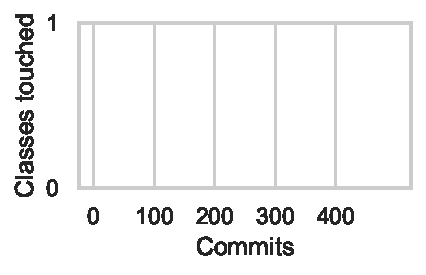
\includegraphics[width=\textwidth]{sections/results/classes/time_series_components_touched.classes.transient.later.joiner.commits_500.pdf}
    \caption{Transient later joiner (n=15304, $\mu$=1.0, median=1.0 \& std=0.0)}
    \label{figure.sections/results/classes/time_series_components_touched.classes.transient.later.joiner.commits_500.pdf}
  \end{subfigure}
\vspace{3mm}
  \begin{subfigure}[b]{0.45\textwidth}
    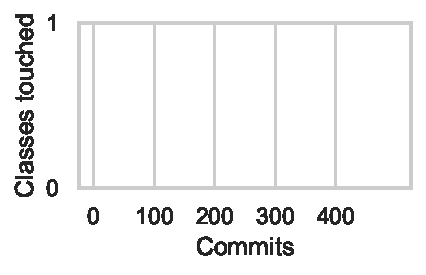
\includegraphics[width=\textwidth]{sections/results/classes/time_series_components_touched.classes.moderate.founder.commits_500.pdf}
    \caption{Moderate founder (n=41, $\mu$=1.0, median=1.0 \& std=0.0)}
    \label{figure.sections/results/classes/time_series_components_touched.classes.moderate.founder.commits_500.pdf}
  \end{subfigure}
  \begin{subfigure}[b]{0.45\textwidth}
    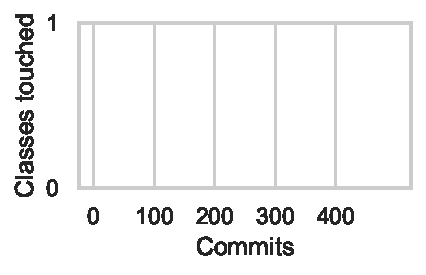
\includegraphics[width=\textwidth]{sections/results/classes/time_series_components_touched.classes.moderate.later.joiner.commits_500.pdf}
    \caption{Moderate later joiner (n=646, $\mu$=1.0, median=1.0 \& std=0.0)}
    \label{figure.sections/results/classes/time_series_components_touched.classes.moderate.later.joiner.commits_500.pdf}
  \end{subfigure}
\vspace{3mm}
  \begin{subfigure}[b]{0.45\textwidth}
    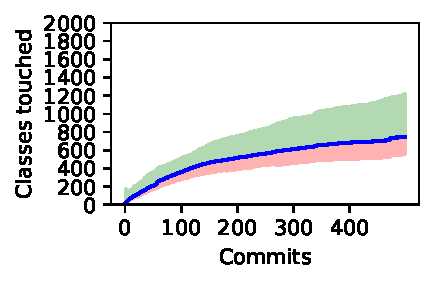
\includegraphics[width=\textwidth]{sections/results/classes/time_series_components_touched.classes.sustained.founder.commits_500.pdf}
    \caption{Sustained founder (n=34, $\mu$=1.0, median=1.0 \& std=0.0)}
    \label{figure.sections/results/classes/time_series_components_touched.classes.sustained.founder.commits_500.pdf}
  \end{subfigure}
  \begin{subfigure}[b]{0.45\textwidth}
    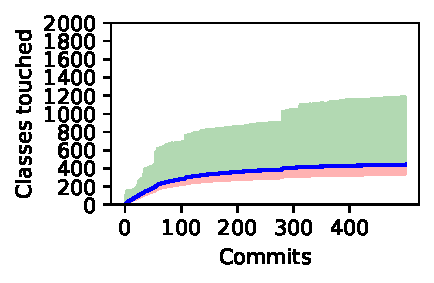
\includegraphics[width=\textwidth]{sections/results/classes/time_series_components_touched.classes.sustained.later.joiner.commits_500.pdf}
    \caption{Sustained later joiner (n=203, $\mu$=1.0, median=1.0 \& std=0.0)}
    \label{figure.sections/results/classes/time_series_components_touched.classes.sustained.later.joiner.commits_500.pdf}
  \end{subfigure}
\caption{A time series for the all commits, excluding transient, with the average mean (blue line), classes touched (y-axis) against the number of commits (x-axis) for six (6) developer categories. Green is the standard deviation above the mean, and pink is the standard deviation below the mean.} 
\end{figure}
\clearpage 
\begin{figure}
  \centering 
  \begin{subfigure}[b]{0.45\textwidth}
    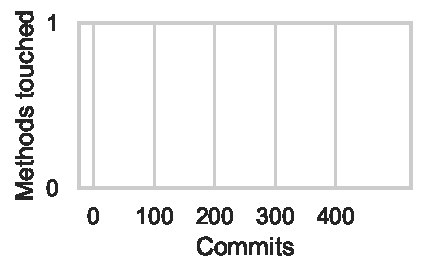
\includegraphics[width=\textwidth]{sections/results/methods/time_series_components_touched.methods.transient.founder.commits_500.pdf}
    \caption{Transient founder (n=206, $\mu$=1.0, median=1.0 \& std=0.0)}
    \label{figure.sections/results/methods/time_series_components_touched.methods.transient.founder.commits_500.pdf}
  \end{subfigure}
  \begin{subfigure}[b]{0.45\textwidth}
    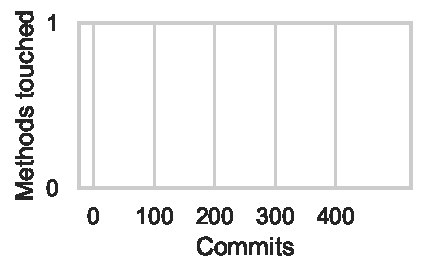
\includegraphics[width=\textwidth]{sections/results/methods/time_series_components_touched.methods.transient.later.joiner.commits_500.pdf}
    \caption{Transient later joiner (n=15304, $\mu$=1.0, median=1.0 \& std=0.0)}
    \label{figure.sections/results/methods/time_series_components_touched.methods.transient.later.joiner.commits_500.pdf}
  \end{subfigure}
\vspace{3mm}
  \begin{subfigure}[b]{0.45\textwidth}
    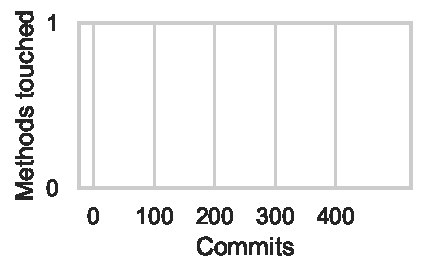
\includegraphics[width=\textwidth]{sections/results/methods/time_series_components_touched.methods.moderate.founder.commits_500.pdf}
    \caption{Moderate founder (n=41, $\mu$=1.0, median=1.0 \& std=0.0)}
    \label{figure.sections/results/methods/time_series_components_touched.methods.moderate.founder.commits_500.pdf}
  \end{subfigure}
  \begin{subfigure}[b]{0.45\textwidth}
    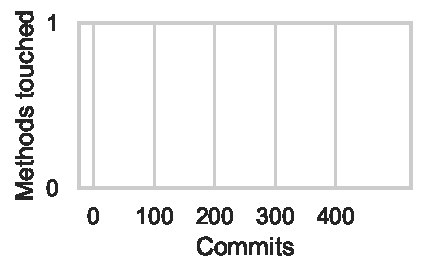
\includegraphics[width=\textwidth]{sections/results/methods/time_series_components_touched.methods.moderate.later.joiner.commits_500.pdf}
    \caption{Moderate later joiner (n=646, $\mu$=1.0, median=1.0 \& std=0.0)}
    \label{figure.sections/results/methods/time_series_components_touched.methods.moderate.later.joiner.commits_500.pdf}
  \end{subfigure}
\vspace{3mm}
  \begin{subfigure}[b]{0.45\textwidth}
    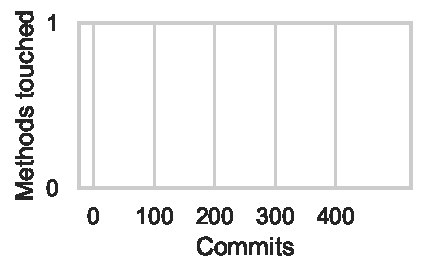
\includegraphics[width=\textwidth]{sections/results/methods/time_series_components_touched.methods.sustained.founder.commits_500.pdf}
    \caption{Sustained founder (n=34, $\mu$=1.0, median=1.0 \& std=0.0)}
    \label{figure.sections/results/methods/time_series_components_touched.methods.sustained.founder.commits_500.pdf}
  \end{subfigure}
  \begin{subfigure}[b]{0.45\textwidth}
    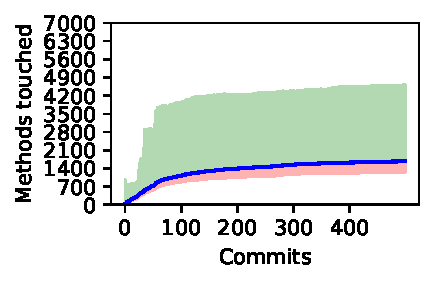
\includegraphics[width=\textwidth]{sections/results/methods/time_series_components_touched.methods.sustained.later.joiner.commits_500.pdf}
    \caption{Sustained later joiner (n=203, $\mu$=1.0, median=1.0 \& std=0.0)}
    \label{figure.sections/results/methods/time_series_components_touched.methods.sustained.later.joiner.commits_500.pdf}
  \end{subfigure}
\caption{A time series for the all commits, excluding transient, with the average mean (blue line), methods touched (y-axis) against the number of commits (x-axis) for six (6) developer categories. Green is the standard deviation above the mean, and pink is the standard deviation below the mean.} 
\end{figure}
\clearpage 
